In the very beginning of the project, most communication was done in full-group meetings. This format worked because the questions discussed were relevant to everyone involved. Over time, it was found that having everyone participate in meetings added a lot of overhead and so it was decided to split the project into subgroups of approximately 5 members.
\begin{figure}[hb]
    \centering
    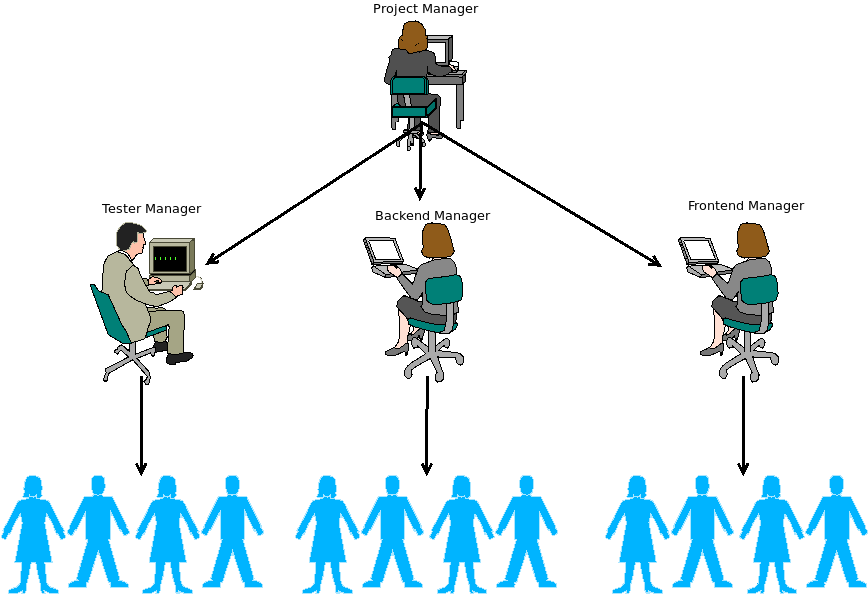
\includegraphics[width=.8\linewidth]{img/group_structure_1.png}
    \caption{The planned project group stucture, here depicting the last of the groupings.}
\end{figure}

For instance, during the pre-study, there was one group that conducted interviews, another group that studied the literature around gamification and so on. By dividing the project group into smaller parts with leaders for each group, some members could be made responsible for managing inter-group communication and management, while the others focused on their work. Above all groups, a project leader was elected to lead the project forward, manage groups and assist the groups in tough design decisions.

Over time, there were some different groupings made to reflect the work that was to be done:
\begin{enumerate}
    \item No groups.
    \item Interviews, platform evaluation and literature studies.
    \item Workshop, framework evaluation, continued platform evaluation. % TODO: I don't remember theese 100%, if someone could fill this in would be great
    \item Tester, backend and frontend.
\end{enumerate}
In some of the groups---such as frontend, backend and tester---there were elected leaders, whereas other groups simply presented their progress to the group when they were done.
